\section{Architectural Description} % (fold)
\label{sec:Architectural Description}

In the following we will be describing the current software architecture for our system. An architectural description could be used as a basis for stakeholder communication, as part of an on-going software design process or to evaluate different architectures \cite{christensen}. In the following we will be using the recommendations found in \cite{christensen} to describe the software architecture. In particular we will be using different viewpoints to communicate the overall structure of the system. In the following we will be looking at the model, C\&C view respectively, we will not be looking at the deployment view in our case, as our system is simple enough that this view would not add much to an overview.

\subsection{Model View}

First we will take a look at the model view. Here we have chosen to jump straight to a mix of package and class diagram as our structure is relatively simple. The class diagram can be seen in figure \ref{mv} below.

\begin{figure}[h!]
  \centering
    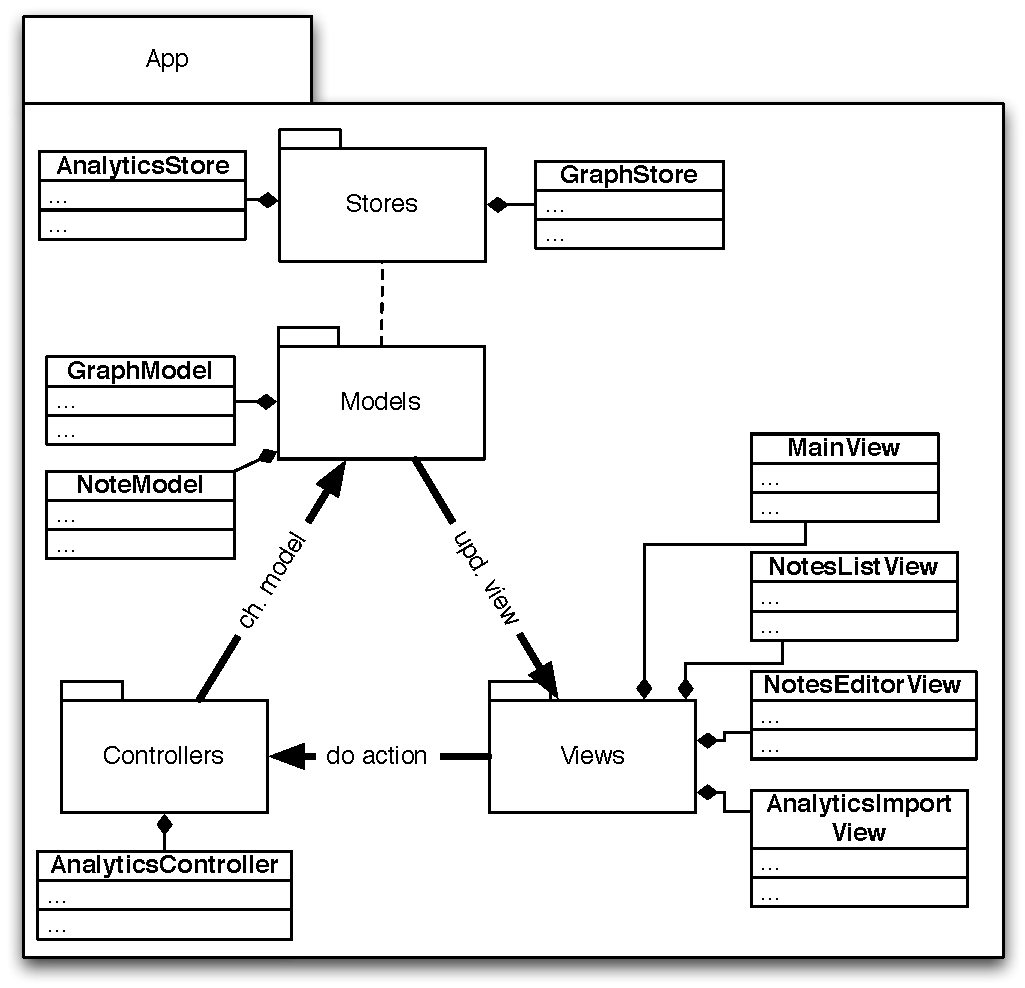
\includegraphics[width=0.66\textwidth]{images/model_view.pdf}
  \caption{Class diagram showing the model view.}
  \label{mv}
\end{figure}

As the class diagram in figure \ref{mv} shows we have a basic MVC architecture, with a storage package which relates closely to the model. In short, the views package contains our different views allowing the user to interact with the system. Actions performed by the user are detected and handled by the controller, which performs a corresponding change to the appropriate model. Finally, the view is updated to reflect the change in the model. 

\subsection{C\&C View}

Next, we have the component and connector view (C\&C), here illustrated using a sequence diagrams as seen in figure \ref{cc} below. Here we have chosen two central functions, in order to show the functional behaviour of certain components and the communication done between them.

\begin{figure}[h!]
  \centering
    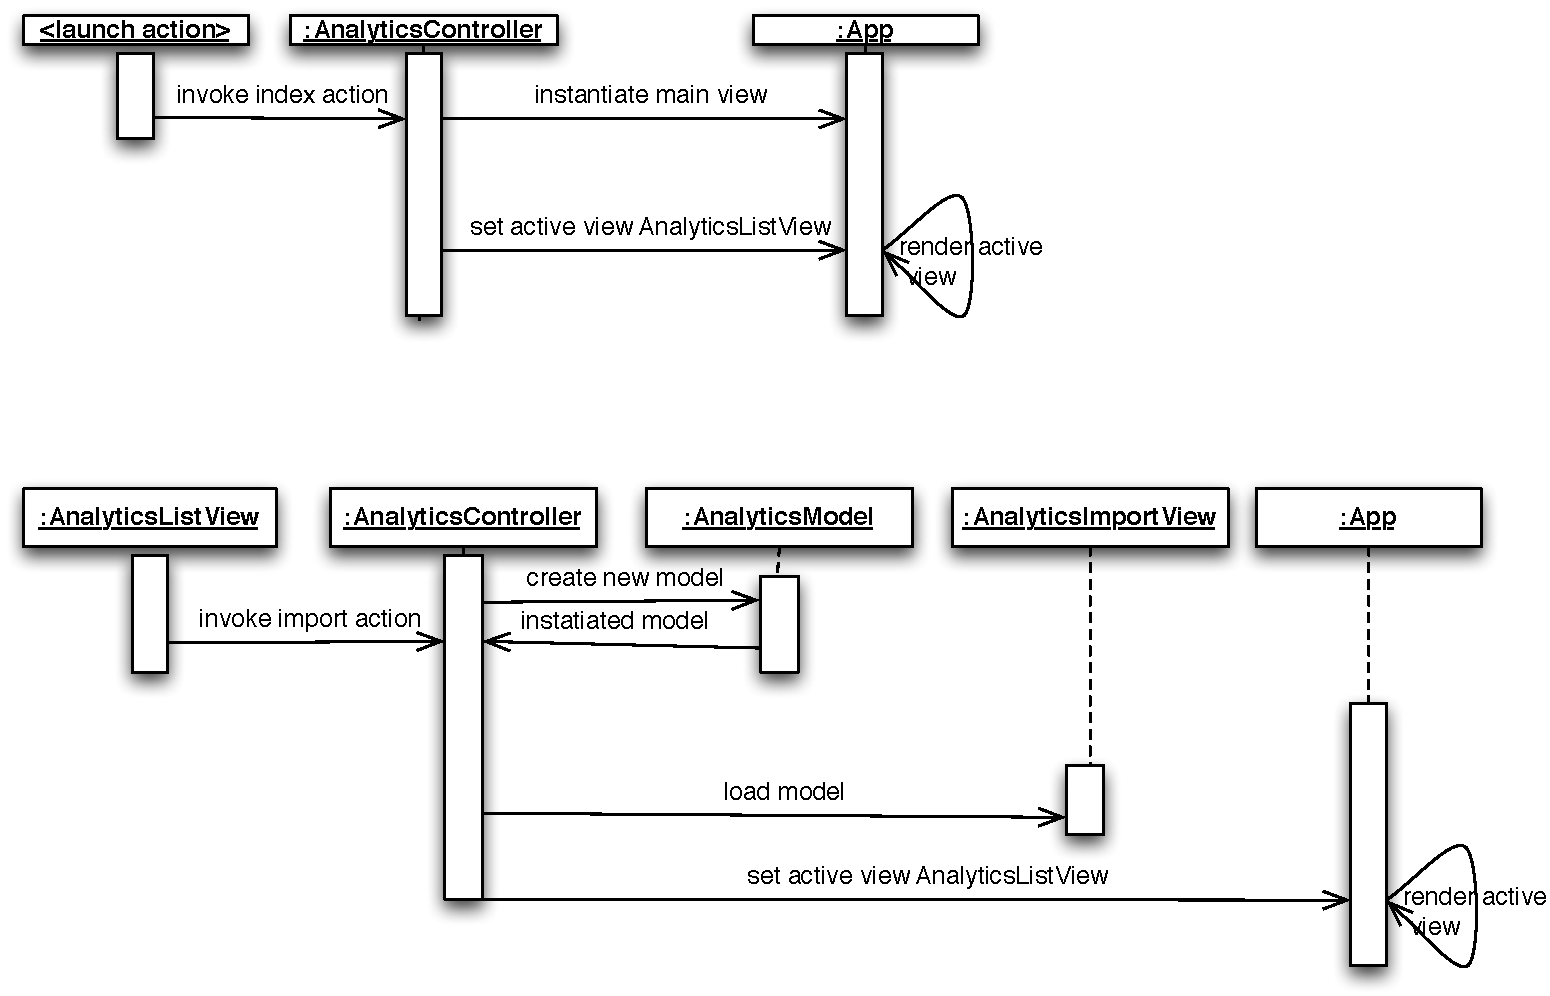
\includegraphics[width=1.0\textwidth]{images/cc_view.pdf}
  \caption{Sequence diagram illustrating the C\&C view.}
  \label{cc}
\end{figure}

The top sequence of figure \ref{cc} illustrates the sequence which occurs when the system itself is launched. When launching, an index action is performed. The controller handles this by instantiating the main view and setting the view to the AnalyticsListView, which the App finally renders.

The bottom sequence of figure \ref{cc} illustrates the sequence which occurs when import action is invoked. First, the controller creates a new model which is loaded into the import view. Then the view is changed and the App renders the active view. 

% section Architectural Description (end)